%   Filename    : chapter_3.tex 
\chapter{Research Methodology}
This chapter lists and discusses the specific steps and activities performed by the researchers in developing Ha.Zee.

\section{Technologies Used}

\subsection{Software}

\subsubsection{Roboflow}
According to Bhattacharyya \citeyear{Bhattacharyya_2020}, Roboflow is a " computer vision developer framework for better data collection to preprocessing, and model training techniques". Roboflow also offers a suite  of browser applications to preprocess and preparation of the data for computer vision and machine learning. Roboflow annotation will be used  to manually set bounding boxes for model training and image augmentation for the manipulation of images \cite{roboflow}.

\subsubsection{Jupyter Notebook using Google Colab and Python}
Jupyter Notebook and Python will be used for training and fitting the data. Jupyter notebook, using google colab,  offers free GPU with CUDA for processing, and Python, the programming language, offers essential libraries for machine learning \cite{googlecolab}.

\subsubsection{A case  for YOLOv5}
Yolov5 is a pre-trained algorithm that uses a system of grids to detect objects from images or videos (https://docs.ultralytics.com/). This tool will be used for the vehicle detection in this project. 

	YOLOv5 is one of the commonly used algorithm for object detection. It is faster than other object detection algorithms like Region-based Convolutional Neural Networks (RCNN), Fast RCNN, and Faster RCNN. Gandhi \citeyear{gandhi_2018} wrote in an article the comparison between the RCNN algorithms and YOLOv5. He said that the major drawbacks of RCNN are that it classifies 2000 regions per image every time it runs, it cannot run in real time and it is a fixed algorithm. Fast RCNN employs a similar algorithm to RCNN but instead of classifying regions everytime, it uses CNN to generate a convolutional feature map where the bounding regions are derived. Faster RCNN improves upon this by using a different network for predicting the regions of the proposal. In his comparison, he found that Fast RCNN improves on the speed of RCNN significantly. He also mentioned that Faster RCNN, the fastest of the RCNN algorithms, is viable for real-time object detection. 
	
	Using the comparison table, Figure \ref{fig:compar_table} from A et al. \citeyear{RAMYA} it was found that YOLOv5 performs the best when it comes to metrics such as Precison, Recall, and Accuracy, although it was mentioned that it is slower to train than version 3 and 4. However, concerning the detection of vehicles for pollutant estimation the researcher put more more emphasis on having better metrics. 
	
	\begin{figure}[!htbp]
		\centering
		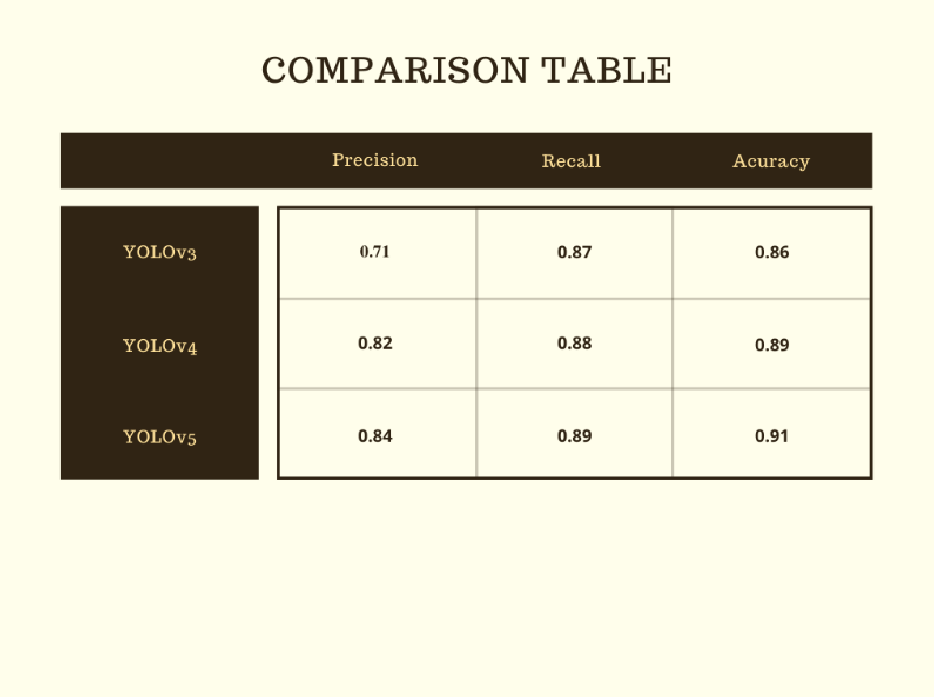
\includegraphics[scale=0.4]{compar_table.png}
		\caption{Comparison table of Precision, Recall, and Accuracy for YOLOv3, YOLOv4, and YOLOv5}
		\label{fig:compar_table}
	\end{figure}
	\FloatBarrier



Ultralytics (https://ultralytics.com/) provides extensive documentation of YOLOv5. This is one of the factors that affect the decision of using YOLOv5 for the study.



\subsection{Hardware}

\subsubsection{Smartphone Cameras}
The study used the built-in cameras of the researchers' smartphones to record the roads and their vehicles. One of the phones has a 48 MP main camera while the other has a 13 MP main camera. Both cameras are able to record 1080p quality videos at 1920 x 1080 dimensions and 30 frames per second (fps).

\subsubsection{Computer}
The computer used in the study runs on 11th Gen Intel, i5-1135G7 (8) @4.200GHz; an NVIDIA GeForce MX450; 8GB of RAM; on an Endeavour x86\_64 OS. The computer utilized CUDA cores to help in the training process.

\section{Research Activities and Development}

\subsection{Development Flow}
There are several processes invloved in developing the object detection model. As shown in Figure \ref{fig:devFlow}, the development consists of several key stages: data gathering, annotation, training, testing, and estimation.

\begin{figure}[!htbp]
	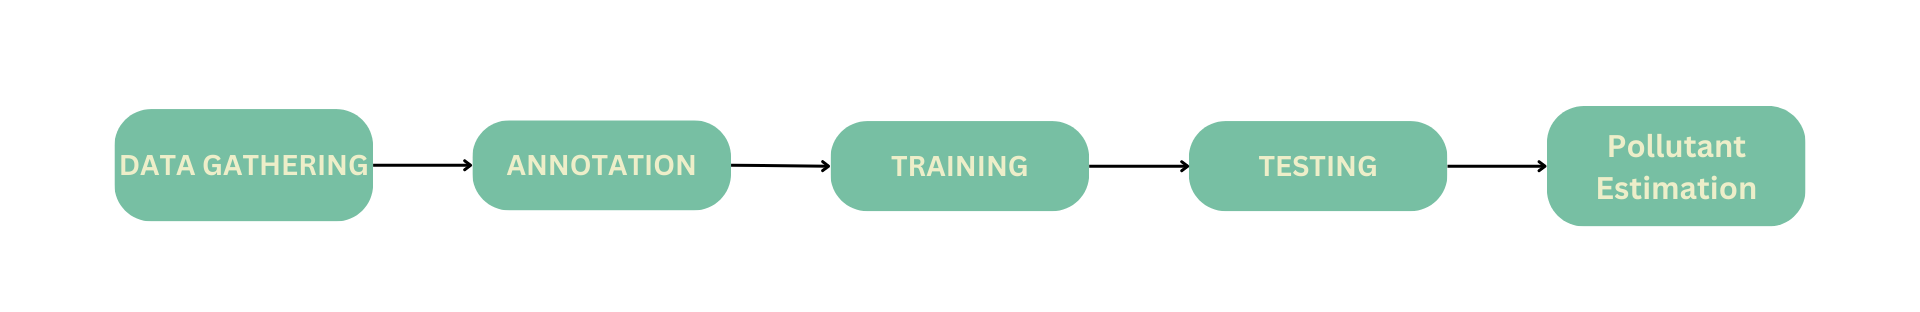
\includegraphics[width=\linewidth]{devFlow.png}
	\caption{Diagram illustrating the flow of the development of the object detection model.}
	\label{fig:devFlow}
\end{figure}
\FloatBarrier

Data gathering involved capturing image and video data from road traffic. Annotation is the process of marking bounding boxes on the captured image data to indicate the objects of interest. Training involves allowing the algorithm to learn and detect the specified objects using the annotated dataset. Testing was done to evaluate the performance of the trained model. Finally, estimation utilized the trained model to estimate the emissions produced by vehicles.


\subsection {Data Gathering}
This study planned to estimate an area’s pollution level through calculating average of the emissions coming from the cars on the road. In doing so, data of the vehicles, its identification, and its emission rates were needed for the study. Through the use of a camera, footage of the vehicles in traffic were recorded to gather the data of vehicles in traffic. This was utilized in training and testing for the software to recognize the vehicles on the video feed. The vehicle emissions values were taken from a study by Rito et al. \citeyear{rito_lopez_biona_2021}.

\subsubsection{Dataset}

Due to the study being conducted in the country of the Philippines, vehicles such as the local jeepney and tricycle do not have readily available image datasets. Videos and images of said vehicles in traffic were taken from different angles using a phone camera. 

Figure \ref{fig:vehicle_samples} show sample images of the different vehicle classes included in the dataset. All images of the vehicles shown were taken by the researchers

\begin{figure}[!htbp]
	\begin{minipage}{1\textwidth}
		\centering
		\subfloat[][Tricycles]{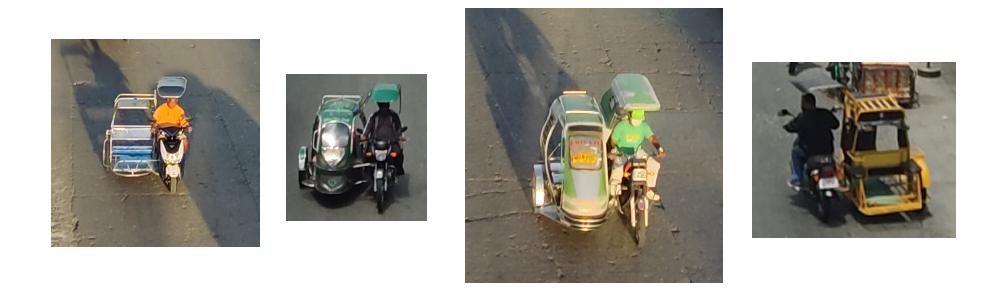
\includegraphics{tricycle_samples.png}}
		
		\subfloat[][Motorcycles]{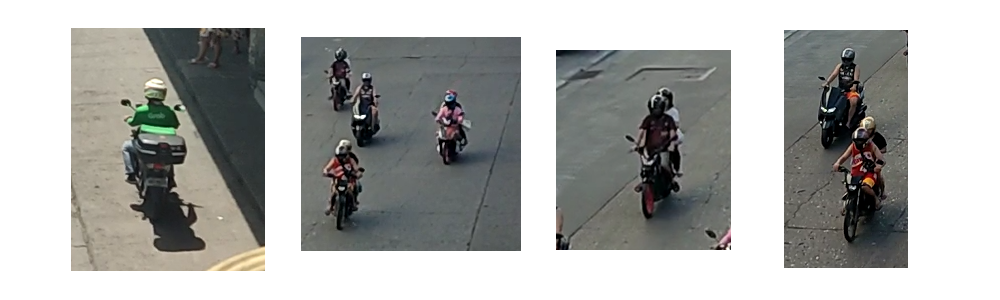
\includegraphics{motor_samples.png}}\\
		
		\subfloat[][Jeepneys]{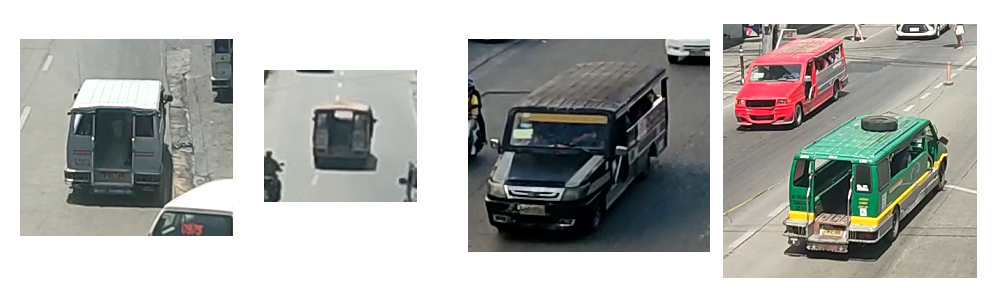
\includegraphics{jeepney_samples.png}}\\
		
		\subfloat[][Cars]{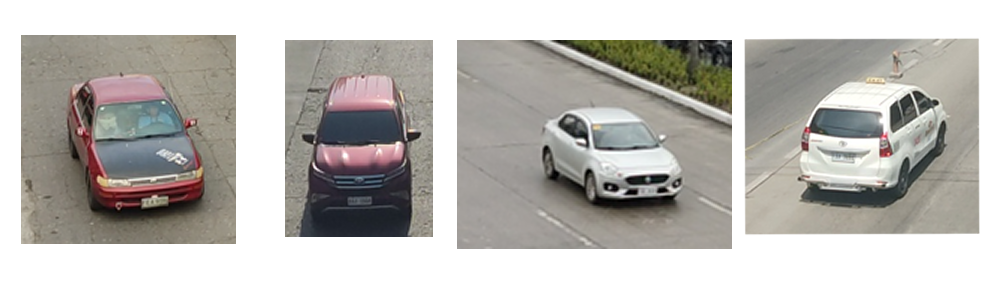
\includegraphics{car_samples.png}}\\
		
		\subfloat[][Utility Vehicles]{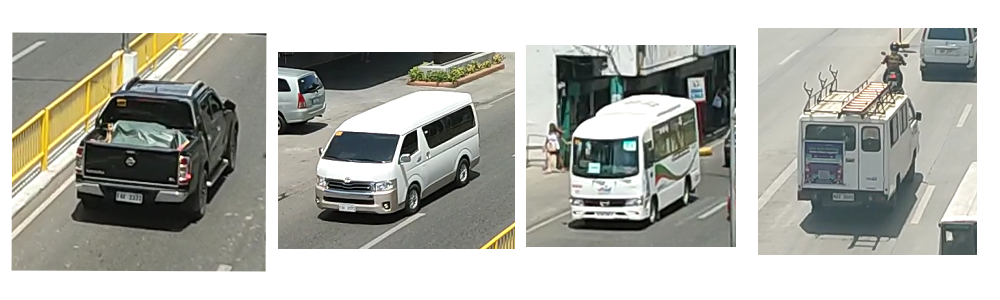
\includegraphics{uv_samples.png}}\\
		
		\subfloat[][Trucks]{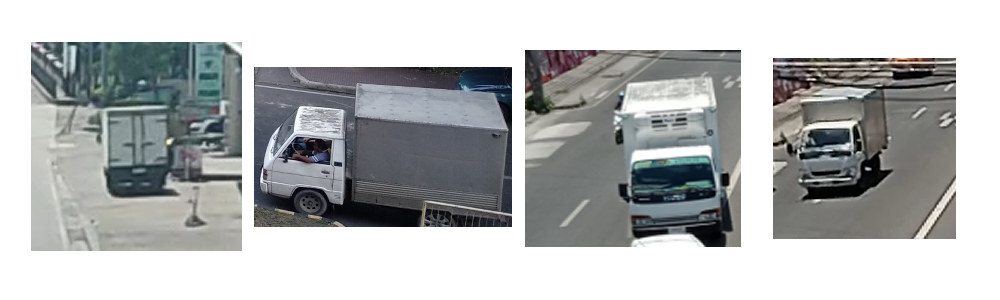
\includegraphics{truck_samples.png}}\\
		
	\end{minipage}
	\caption{Sample images of vehicles used in the study}
	\label{fig:vehicle_samples}
\end{figure}
\FloatBarrier

\subsubsection{Class Distribution}
Taken from Roboflow's "health check report", Figure \ref{fig:class_bal} depicts the distribution of the various classes after collecting data and annotating images. The dataset only contains data taken by the researchers.

\begin{figure}[!htbp]
	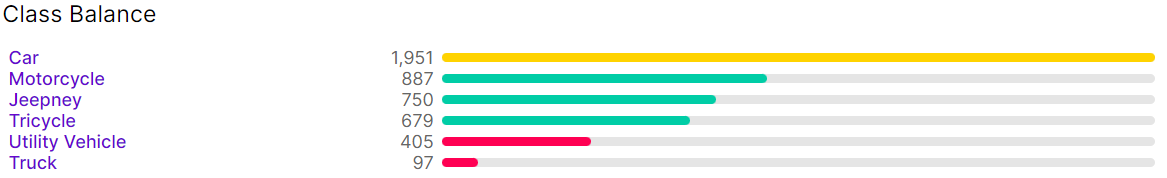
\includegraphics[width=\linewidth,scale=0.8]{class_balance.png}
	\caption{Graph of class balance between the six vehicle types}
	\label{fig:class_bal}
\end{figure}
\FloatBarrier

The class with the highest number of samples in Figure \ref{fig:class_bal} is the "Car" class, comprising 1951 samples. Notably, the "Car" class is twice as abundant as the second-ranked class, "Motorcycle." This disparity in sample counts can be attributed to the abundance of "Car" objects at the locations where the data were collected.
In contrast, the "Truck" class exhibits the lowest number of samples in the dataset, with only 97 instances captured. The scarcity of "Truck" samples suggests that this class is relatively less represented compared to other classes within the dataset.

Such disparities in sample distribution across classes can have implications for model training and performance, as it may impact the ability of the model to accurately classify and detect objects from underrepresented classes or overrepresented classes might overfit the data.



\subsection {Preprocessing and Annotation}

	Preprocessing the data includes defining the bounding box of the vehicles in the training data and augmenting the images to make the model perform better. Roboflow has an annotation tool that can be used for  training the model to detect a vehicle in an image and its type. Augmentation of the images will be done by the YOLOv5 algorithm automatically given that the Albumentation library is installed. According to Dilmegani \citeyear{dilmegani}, Augmentation can be used for transforming the images allowing the model to diversify its training data set making it perform better.
	

	
\subsubsection{Annotation Method}
Annotation of the vehicles consist of: full image annotation and vehicle cropping. In full image annotation, the entire image or video frame is used and every vehicle present is then selected and categorized for the Roboflow tool to save. Vehicle cropping is when a vehicle/small group of vehicles is/are cropped from the source image/video frame and is then annotated by the tool. This was done when a specific type of vehicle was needed for the database. The training data was separated into different classes and was also the bases of classification for the training: cars, jeepneys, motorcycles, tricycles, trucks, and utility vehicles. 

Figure \ref{fig:full_img_anno} shows the full image annotation, wherein every bounding box is color coordinated to the type of vehicle used in the study.

\begin{figure}[!htbp]
	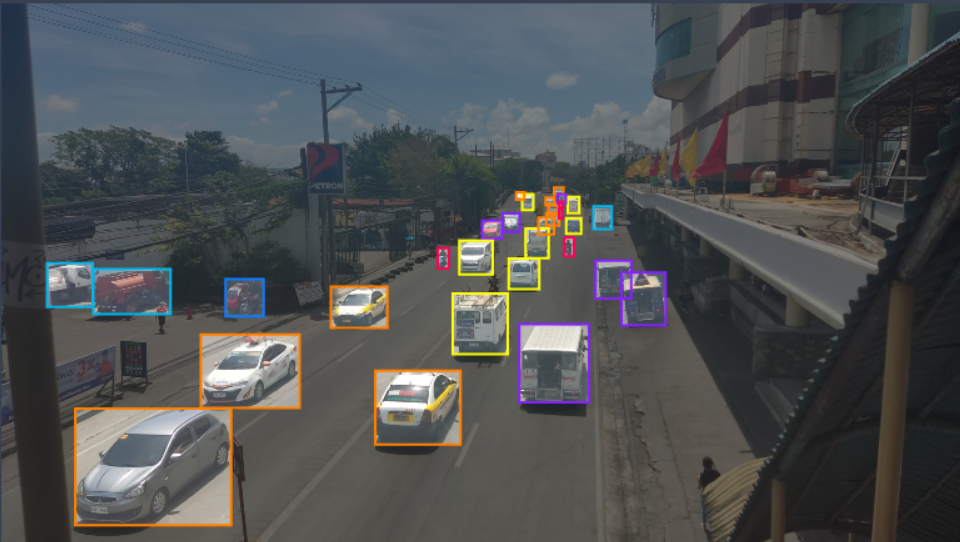
\includegraphics[width=\linewidth]{full_img_anno.png}
	\caption{Full image annotation of vehicles in Gaisano City, Luna St., Lapaz, Iloilo City in Roboflow}
	\label{fig:full_img_anno}
\end{figure}
\FloatBarrier

Figure \ref{fig:cropped_anno} uses a vehicle cropping method. In this specific example, the researchers needed more data of the tricycle. Hence, samples of tricycles over different images/frames from videos were cropped before being uploaded to the Roboflow annotation tool. 

\begin{figure}[!htbp]
	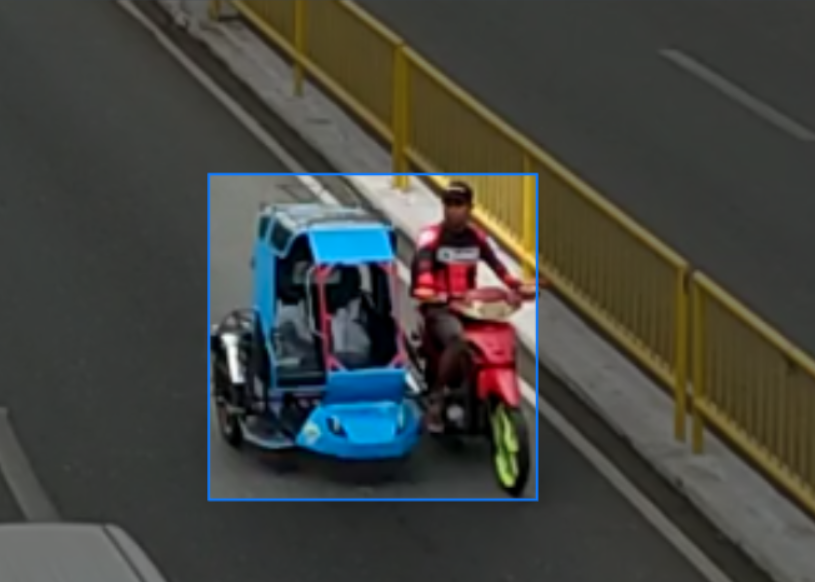
\includegraphics[width=\linewidth]{cropped_anno.png}
	\caption{Image of motorcycle cropped before being annotated in Roboflow}
	\label{fig:cropped_anno}
\end{figure}
\FloatBarrier

When generated using Roboflow, the dataset undergoes preprocessing steps to optimize training efficiency. Firstly, the images are resized to a dimension of 640x640, facilitating faster training. Additionally, the pixel order is adjusted to ensure proper alignment. To enhance performance with smaller objects, the mosaic augmentation technique is applied. The result of this preprocessing is a directory comprising the train, validation, and testing images, accompanied by the necessary "data.yaml" file, necessary for YOLOv5 training.


\newpage

\subsection {Training and Performance Testing}
The training was done using Google Colab which offers GPU compute that has CUDA available. To prevent CUDA from running out of memory during the training process of the model, the researchers opted to use 16 batches which provides enough memory per batch and also ensured that the training will not be interrupted by memory-related issues involving CUDA. Furthermore, in consideration of the time constraints and to prevent potential overfitting, the final model was trained for 100 epochs for approximately three hours using the weights obtained from a previous version of the dataset for transfer learning. The previous version was trained for 300 epochs using the yolov5x.pt pre-trained checkpoint, and was trained for approximately six hours. The trained checkpoint yolov5x.pt was used because the dataset collected was small compared to the recommended number of data \cite{Jocher_Waxmann_2022} and is expected to perform better when using transfer learning than to be trained from scratch \cite{Lihi_Gur_Arie_2023}.

The values of the hyperparameters that was used during the training are shown in Table \ref{tab:hyperparameters} . The values presented are the default value of the hyperparameters of YOLOv5.

\begin{table}[ht]   %t means place on top, replace with b if you want to place at the bottom
	\centering
	\caption{Table of the YOLOv5 hyperparameters used during training} \vspace{0.25em}
	\begin{tabular}{c|c|c|c|c|c} \hline
		\centering \textbf{Hyperparameter} & \textbf{Value} &\textbf{Hyperparameter} & \textbf{Value} & \textbf{Hyperparameter} & \textbf{Value} \\ \hline
		lr0  & 0.01   & obj & 1.0 & scale &0.5 \\
		lrF  & 0.01   & obj\_pw & 1.0 & shear &0.0 \\
		momentum  & 0.937   & iou\_t & 0.2 & perspective &0.0 \\
		weight\_decay  & 0.0005  & anchor\_t & 4.0 & flipud &0.0 \\
		warmup\_epochs  & 3.0  & fl\_gamma & 1.0 & scale &0.5 \\
		warmup\_momentum  & 0.8   & hsv\_h & 0.015 & mosaic &1.0 \\
		warmup\_bias\_lr  & 0.1   & hsv\_s & 0.7 & mixup &0.0 \\
		box  & 0.05   & has\_v & 0.4 & copy\_paste &0.0 \\
		cls  & 0.5   & degrees & 0.0 &  & \\
		cls\_pw  & 1.0   & translate & 0.1 &  &  \\
		 \hline
		
	\end{tabular}
	\label{tab:hyperparameters}
\end{table}
\FloatBarrier

The hyperparameters were unchanged due to the substantial cost associated with evolving the hyperparameters or conducting trial-and-error experiments. Hyperparameter evolution requires extensive computational resources and is time-consuming (Jocher \& Waxmann, 2023).

Table \ref{tab:hyperparameters} contains the augmentation methods utilized during training. These methods include hsv\_h, hsv\_s, hsv\_v, translate, scale, fliplr, and mosaic. hsv\_h, hsv\_s, and hsv\_v augment the HSV (Hue, Saturation, Value) values, thereby manipulating the color characteristics of an image. Translate allows the image to be shifted along an axis, adjusting its position. Scale controls the size of an image, determining its dimensions. Fliplr horizontally flips the image, creating a mirrored version. Lastly, Mosaic involves combining multiple images to form a single collage-like image. By using these augmentation techniques, the training process improves the diversity and variability of the dataset, ultimately improving the model's ability to generalize and handle various scenarios.

To evaluate the training process and assess the performance of the model during training, YOLOv5 automatically generates graphics and visualizations which are essential in assessing the progression of the model throughout the training phase, as well as providing insights into the performance metrics of the trained model after training. These visualizations aid in deciding whether the model's performance meets the desired value.


\section {Model Application}
The program detect.py was run to detect objects from an external device or video file using the trained model. When detect.py is run it will start to list the objects it detects. An average emission of each vehicle type will be used. The study from Rito et al. \citeyear{rito_lopez_biona_2021} provides a table that quantifies the emission factors of energy consumption of multiple vehicle types, 6 of which are to be used in this study. The emission data from the study will be utilized for the application. Table \ref{tab:emission} shows the grams of emissions per kilometer.
The averages of the vehicles’ $PM_{2.5}$ emissions  at a given time will be displayed on the corner of the video recording and will be periodically updated as vehicles enter and leave the camera’s or video’s line of sight. 

\begin{table}[ht]   %t means place on top, replace with b if you want to place at the bottom
\centering
\caption{Emission factors per vehicle type ($g_{emissions}/km$)} \vspace{0.25em}
\begin{tabular}{p{2in}|c|c|c|c} \hline
\centering \textbf{Vehicle Type} & $PM_{2.5}$ &\ch{CH4} & \ch{N2O} & \ch{CO2} \\ \hline
Tricycle   & 0.0562   & 4.0906 & 0.0021 &  66.8747 \\
Motorcycle& 0.0336  &2.3022   & 0.0015 & 60.0983\\ 
Jeepney &0.8466&0.2357  &0.0316	& 668.7415\\ 
Car & 0.0221 & 0.7408  & 0.0099  & 109.8958\\ 
Utility & 0.1430 & 0.3538 & 0.0063 & 92.4039\\ 
Light Truck & 0.7519 & 0.3648 & 0.0226 & 842.0852\\ \hline

\end{tabular}
\label{tab:emission}
\end{table}

\subsection{Calculating the Pollutant Emission Estimate}

The system, after assigning values to each vehicle, calculated the vehicles’ pollutant emissions using the following equation:
\begin{equation}
\text{vehicle pollutant estimation} = \frac{\sum\text{(total count of vehicle x * vehicle x's pollutant value)}}{\text{Total vehicles detected}}
\end{equation}

The total count of the vehicle x was multiplied to its assigned pollutant value. The sum of the product of every vehicle was then divided by the total number of detected vehicles on the frame to get the average. This results in the estimated pollutant value being produced from vehicles in a current frame.


\section{System Architecture}

A separate system for inference was made to allow the program to count the number of vehicles and approximate emissions. The available program for detection (detect.py) was not used because it was meant to run for general cases and not for videos and webcam footage of vehicles specifically as indicated in the github page for YOLOv5 (https://github.com/ultralytics/yolov5). 

\begin{figure}[!htbp]
	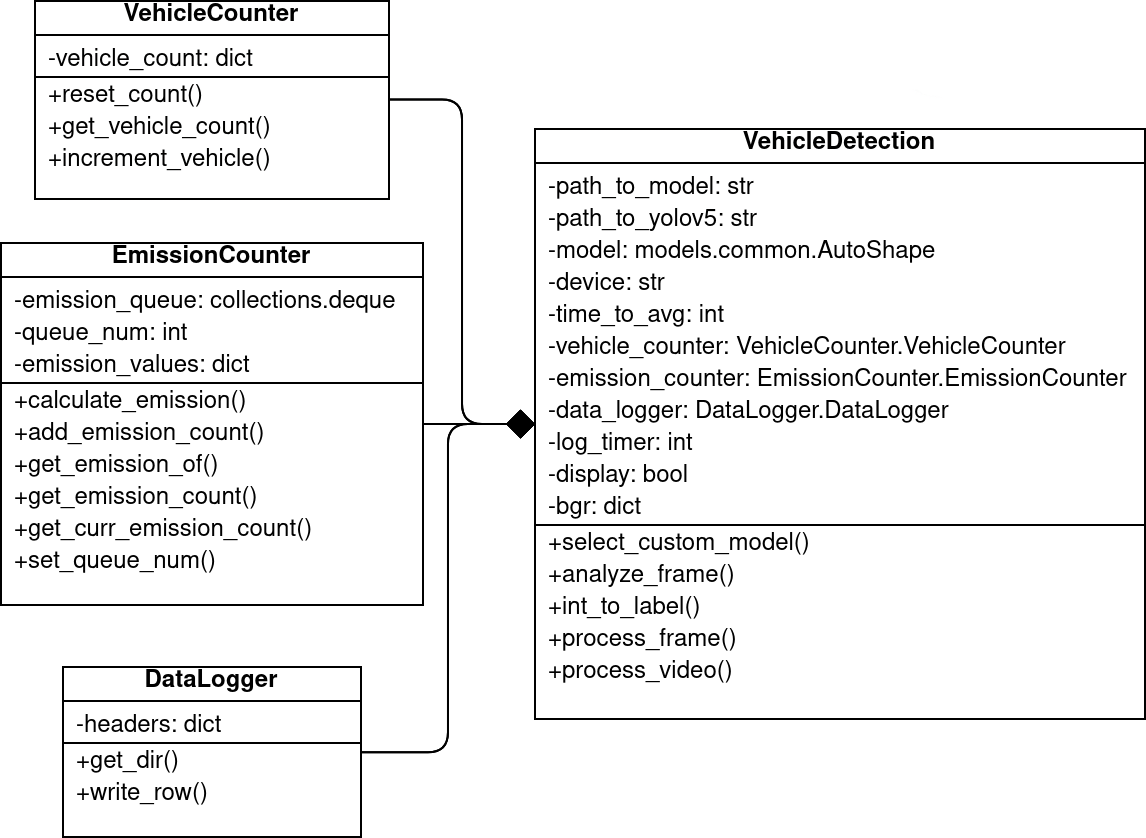
\includegraphics[width=\linewidth]{system_uml.png}
	\caption{UML class diagram of Ha.Zee}
	\label{fig:system_uml}
\end{figure}
\FloatBarrier

The system architecture is displayed in Figure \ref{fig:system_uml} , consisting of four distinct classes. The VehicleDetection class plays a central role in vehicle detection and emission counting. It collaborates with three other classes: VehicleCounter, EmissionCounter, and DataLogger. This design ensures that each class has a specific and well-defined role within the system.

The VehicleCounter class serves as a click counter, responsible for tallying the number of vehicles within a single frame. Its primary function is to count vehicles detected in each frame accurately.

The EmissionCounter class stores the emission estimate in a dictionary. This enables the calculation of the average emissions across all video frames. By considering the emissions from every frame equally,an overall average that represents the emissions from the entire video is obtained.

The DataLogger class handles the essential task of logging data into an external CSV file. It ensures systematic recording and storage of relevant information such as the vehicle count and pollutant estimations.

The VehicleDetection class acts as the system backbone, analyzing each video frame. It performs object detection, leveraging the three classes mentioned above to count vehicles, calculate the average emissions of pollutants across all video frames, and export the collected data into a CSV file.

The creation of the aforementioned classes ensures a distinction of goals, allowing each class to fulfill its designated function effectively within the system. As a result, the system achieves proper vehicle detection, estimation of pollutant emissions, and data logging while calculating the average emissions of pollutants across all video frames.


%
%\section{Calendar of Activities}
%
%Table \ref{tab:timetableactivities} shows a Gantt chart of the activities for the development of Hazy.  Each bullet represents approximately
%one week worth of activity.
%
%%
%%  the following commands will be used for filling up the bullets in the Gantt chart
%%
%\newcommand{\weekone}{\textbullet}
%\newcommand{\weektwo}{\textbullet \textbullet}
%\newcommand{\weekthree}{\textbullet \textbullet \textbullet}
%\newcommand{\weekfour}{\textbullet \textbullet \textbullet \textbullet}
%
%%
%%  alternative to bullet is a star 
%%
%\begin{comment}
%   \newcommand{\weekone}{$\star$}
%   \newcommand{\weektwo}{$\star \star$}
%   \newcommand{\weekthree}{$\star \star \star$}
%   \newcommand{\weekfour}{$\star \star \star \star$ }
%\end{comment}
%
%
%%
%\begin{table}[ht]   %t means place on top, replace with b if you want to place at the bottom
%\centering
%\caption{Timetable of Activities} \vspace{0.25em}
%\begin{tabular}{|p{2in}|c|c|c|c|c|c|c|c|c|c|} \hline
%\centering Activities  & Sept  & Oct & Nov & Dec & Jan & Feb & Mar & April & May & June\\ \hline
%Finding and Choosing Final Topic      & ~~~\weektwo &  &  &  &  &  & &&& \\ \hline
%Review of Related Literature &   & \weekfour & \weekfour &  &  &  & & ~~~\weekone& \weekone~~~ & \\ \hline
%Identifying Problem Statement     &  ~~~\weektwo &  \weekone~~~  &  & &  &  &  &&&\\ \hline
%Formation of Possible Solution    &   & ~~~\weektwo  &  \weekone~~~ &  & & & &&&  \\ \hline
%Constructing the Methodology     &   &  &   ~~~\weektwo & \weekthree ~~ & &  & &&& \\ \hline
%
%Documentation & ~~~\weektwo  & \weekfour & \weekfour &\weekone ~~& & ~~~\weektwo &  & ~~~\weektwo & \weekone~~~ & ~~~\\ \hline
%Model Training   &  &  &  & & & & \weekone~~~  & ~~~\weektwo & \weekone~~~  & \\ \hline
%Data Gathering & & & & & &\weekfour&\weekfour& \weekfour & &~~~  \\ \hline
%Testing     &   &  &  & \weekthree ~~ & &  & ~\weekone~ & ~~~\weekone & \weekone~~~ &  \\ \hline
%Interpretation of Results     &   &  &  & \weekthree ~~ & &  & &~~~\weekone& \weekone~~~ & \\ \hline
%
%\end{tabular}
%\label{tab:timetableactivities}
%\end{table}

